\section{Agente Bioinspirado e implementacion}

\begin{frame}{Dinamica Neuronal FIU}
  \begin{columns}[T,onlytextwidth]
    \column{0.50\textwidth}

    % Compactar SOLO las ecuaciones (no toda la slide)
    {\small
    \setlength{\abovedisplayskip}{2pt}
    \setlength{\belowdisplayskip}{2pt}
    \setlength{\jot}{2pt}

    \begin{equation*}
      \begin{aligned}
        S_n &= E_n + \sum_{j=1}^{m} I_{in}^{j}
      \end{aligned}
    \end{equation*}

    \begin{equation*}
      O_n =
      \begin{cases}
        S_n - T_n, & \text{si } S_n > T_n \\
        0,         & \text{en otro caso}
      \end{cases}
    \end{equation*}

    \begin{equation*}
      E_n =
      \begin{cases}
        S_n - T_n, & \text{si } S_n > T_n \\
        E_n - d_n, & \text{si } S_n \le T_n \ \land\  S_n = E_n \\
        S_n,       & \text{en otro caso}
      \end{cases}
    \end{equation*}

    \begin{equation*}
      I_{in}^{j} =
      \begin{cases}
        \ \omega_j O_j, & \text{gap junc. y } O_j \ge E_n \\
        -\omega_j O_j,  & \text{gap junc. y } O_j < E_n \\
        \ \omega_j O_j, & \text{exc. química} \\
        -\omega_j O_j,  & \text{inh. química}
      \end{cases}
    \end{equation*}
    } % end \small

    \column{0.50\textwidth}
    \begin{itemize}
        \item Variables de estado
            \vspace{0.15cm}
            \begin{itemize}
                \item $E_n$: estado interno
                \item $O_n$: estado externo
            \end{itemize}
        \vspace{0.2cm}
        \item Parametos de la dinamica
            \vspace{0.15cm}
            \begin{itemize}
                \item $T_n$: umbral de disparo
                \item $d_n$: factor de decaimiento
            \end{itemize}
    \end{itemize}
    \begin{block}{Desafio}
        Implementar esta dinamica para poder aplicar el descenso por el gradiente y BPTT.        
    \end{block}
  \end{columns}
\end{frame}

\begin{frame}{La arquitectura TWC}
  \centering
    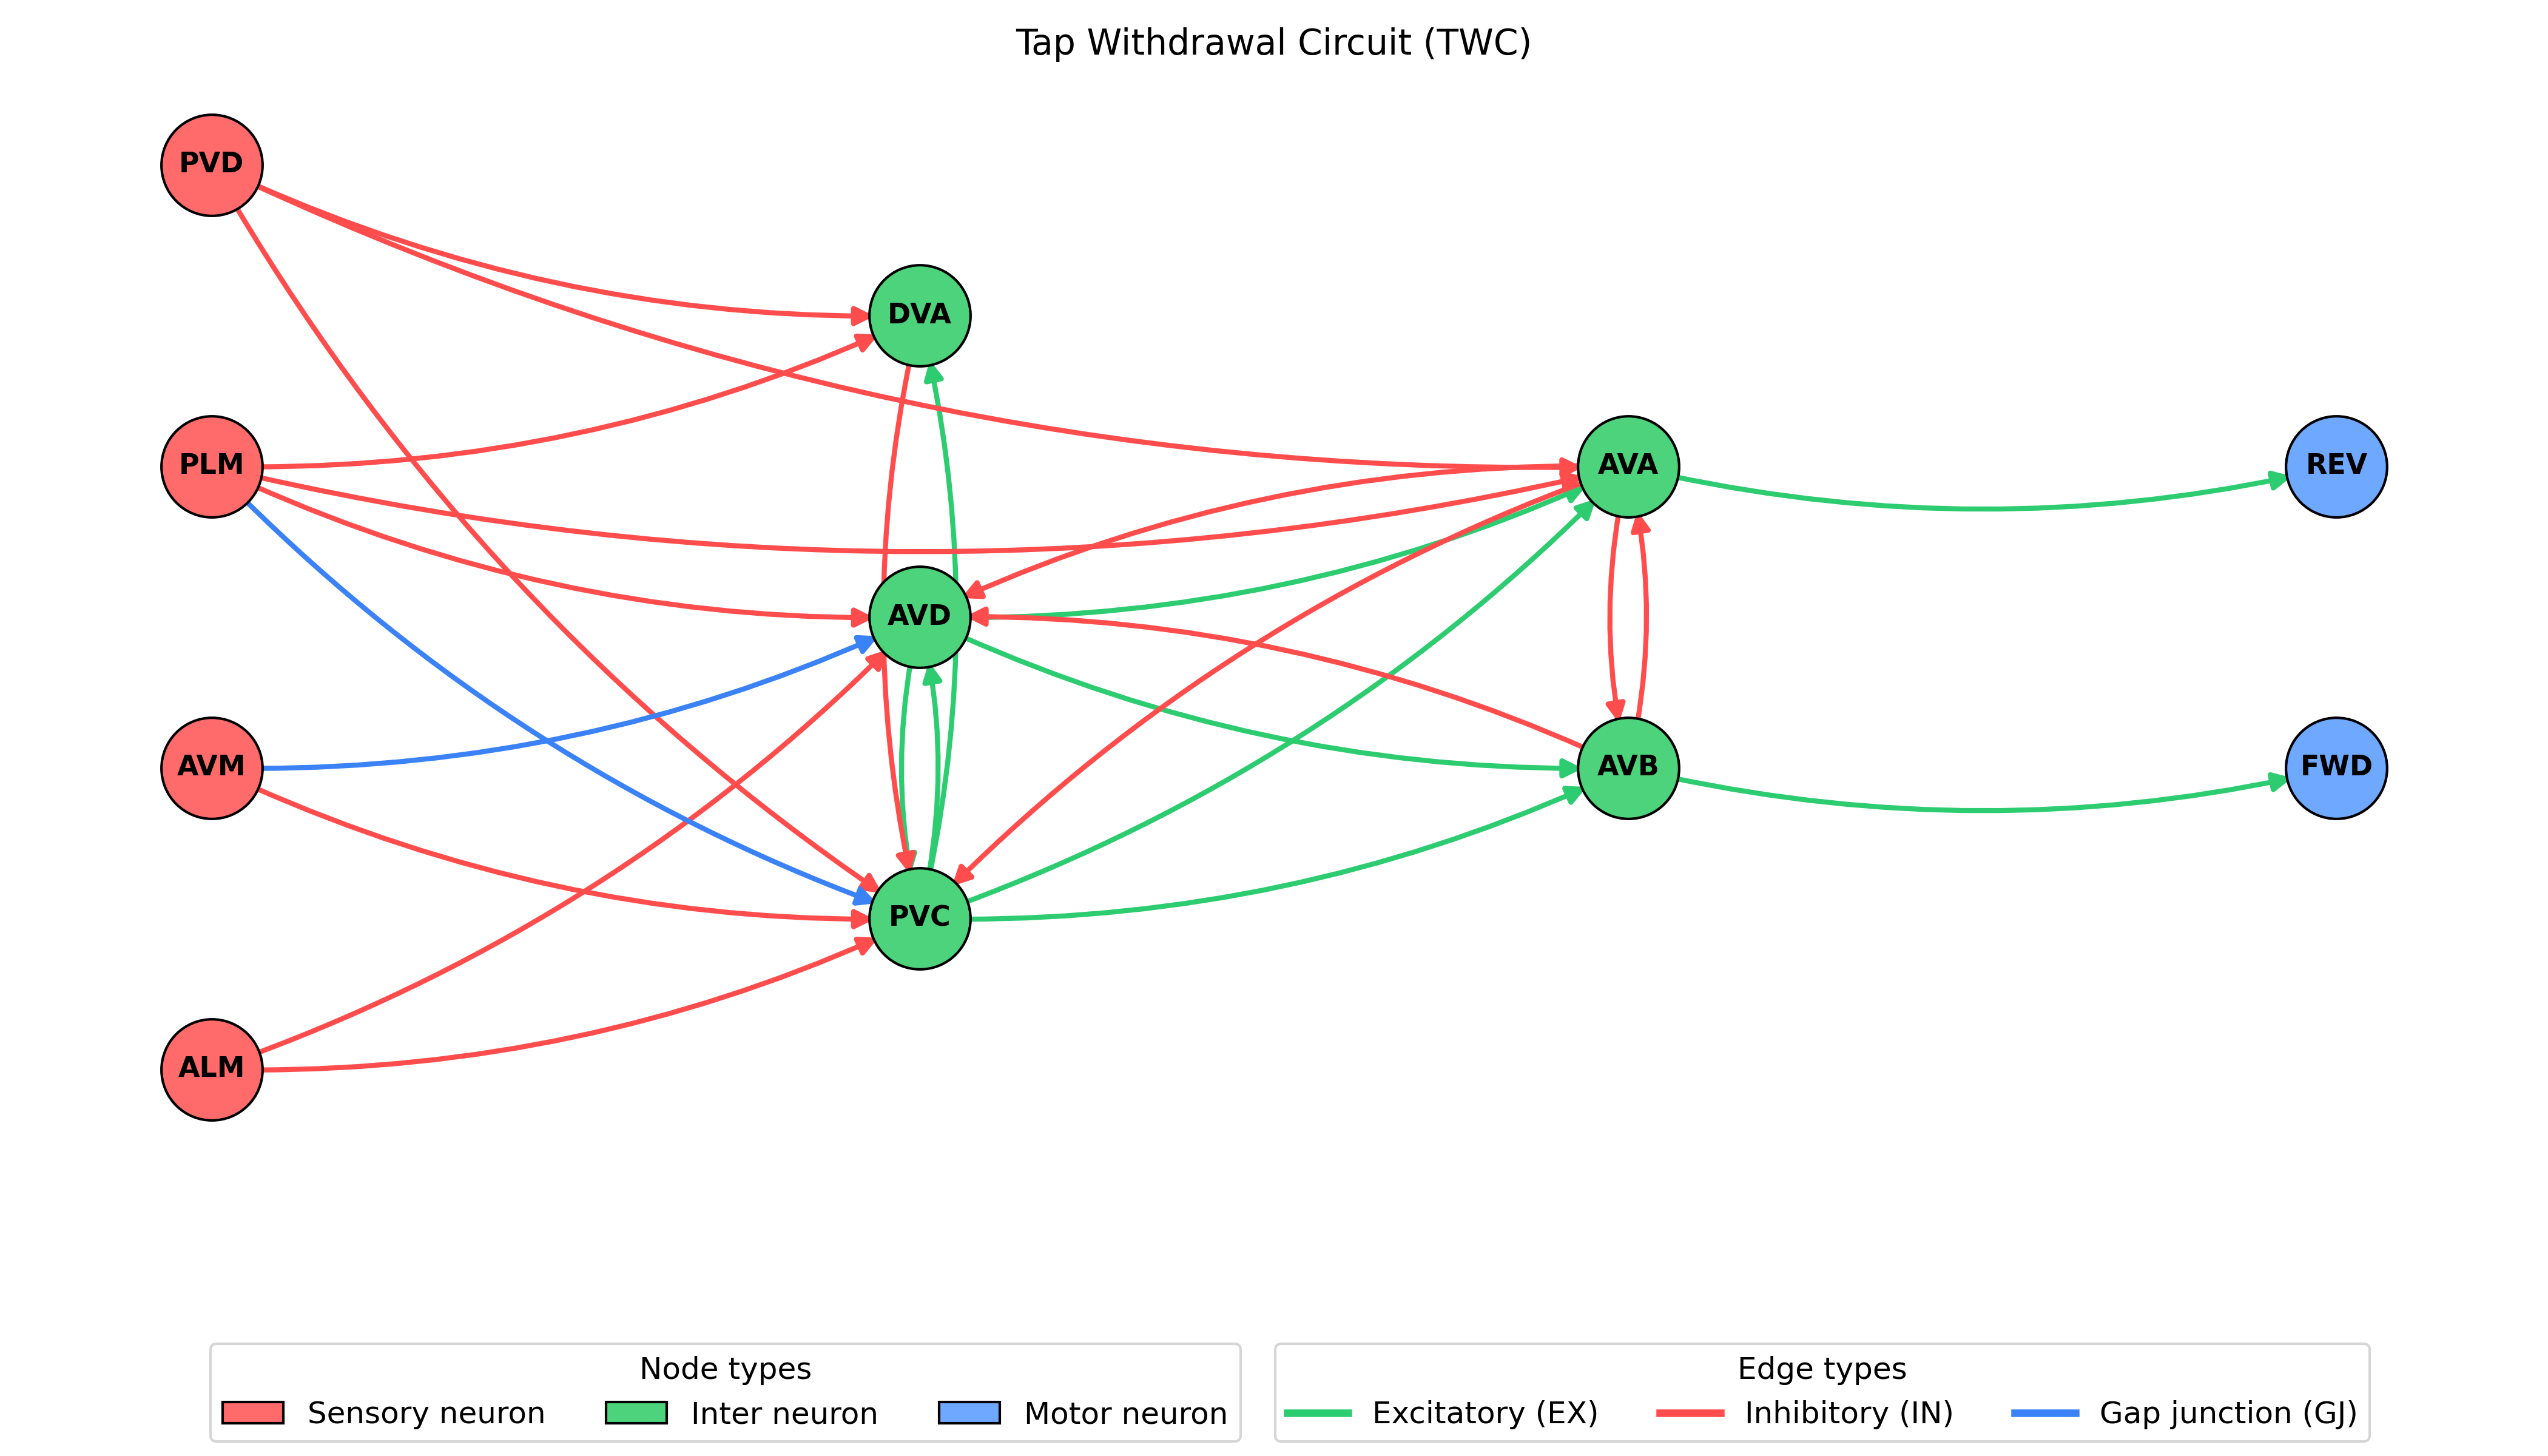
\includegraphics[
      width=\linewidth,
      height=0.82\textheight,
      keepaspectratio
    ]{./attatchments/twc.png}
\end{frame}

\begin{frame}{Implementación del Agente: PyUriTwc}
    \begin{itemize}
        \item Clase personalizada \texttt{PyUriTwc} (\texttt{nn.Module}) compatible con \textit{Autograd} (PyTorch)
        \item Interaccion con el entorno modularizada
        \item Estructura vectorizada para:
            \begin{itemize}
                \item Conexiones y pesos 
                \item Parámetros
                \item Dinámica neuronal
            \end{itemize}
        \item Modos de ejecución:
            \begin{itemize}
                \item \texttt{forward}: interacción (estado persistente)
                \item \texttt{forward\_bptt}: secuencias temporales, utilizado para entrenamiento.
            \end{itemize}
    \end{itemize}
\end{frame}

\begin{frame}{Implementación del Agente: PyUriTwc}
  \begin{columns}[T,onlytextwidth]

    % ---- Columna izquierda: texto ----
    \column{0.50\textwidth}
        \textbf{Topología}: conexiones y pesos representados mediante una unica matriz $11 \times 11$ junto a mascaras binarias para las conexiones sinapticas
        \begin{itemize}
            \item \texttt{mask\_ex}
            \item \texttt{mask\_in}
            \item \texttt{mask\_gj}
        \end{itemize}

    \pause
    % ---- Columna derecha: imagen ----
    \column{0.50\textwidth}
        \textbf{Dinámica Neuronal:}
        \begin{itemize}
            \item Calculo de $(E_{t+1},O_{t+1})$ en simultaneo
            \item $O_n = ReLU(S_n - Th_n)$
            \item $E_n$ reemplazado por operaciones con enmascaramiento. (\texttt{torch.where})
            \vspace{0.1cm}
            $$
            \begin{aligned}    
                E_{new} = &M_{fire} \cdot Val_{fire} + \\
                          &M_{decay} \cdot Val_{decay} + \\
                          &M_{accum} \cdot Val_{accum}
            \end{aligned}
            $$
        \end{itemize}

  \end{columns}
\end{frame}
